\documentclass[a4paper, 11pt]{book}
\usepackage{graphicx}
\title{Python for the Under 10's}
\author{Graeme Winter}
\begin{document}
\maketitle
\clearpage
\thispagestyle{plain}
\par\vspace*{.35\textheight}{\centering For Emily, I hope you find
  this fun\par}
\chapter{Introduction}

\section{Preface for Grown Ups}

When the author was a child computers were smaller, simpler and harder
to break\footnote{Machines like the BBC Model B, ZX81 and Spectrum 48k
  spring to mind}, and so much more suitable for leaning how they
work. Today computers are bigger, more complex, easier to break and
much less straightforward to understand. At the same time they are
used for everything: from catching up on TV to reading the news,
communicating with people and games. This has meant that the creative
process of writing simple computer programs (typically games) has been
lost in favour of easily accessed entertainment. While none of this is
a bad thing, it has removed the opportunity to learn \emph{how they
  work}. The idea of this book is to provide this opportunity, using
free tools and real programming languages. 

The pre-requisite for this is a relatively recent computer - anything
bought since about 2005 or so, running Windows, Linux or Mac OS X
should be fine. The only dependency is the installation of Python
2.7.3 or later from http://www.python.org. If you have an old laptop
lying around which used to be useful and is no longer, this will
probably be fine. If you're feeling really keen the Raspberry Pi may
be for you (http://wwww.raspberrypi.org) as this is a little computer
aimed at children learning about computers, which will plug into the
TV in the same way as computers from the mid 1980's did, only much
more powerful... 

\section{Preface for Children}

Most grown ups use computers for a lot of the day, but most of them
have no idea how they work - the idea of this book is to help you
learn how they work and what they can do. Telling the computer what to
do is called programming, and there are lots of different languages
you can use to tell the computer what to do. This book is about one
called Python (yes, like the snake) which is good because it is one of
the easiest and also lets you do fun things straight away. 

In the book the pictures are called ``figures'' and you will find that
they are numbered - when you get to a bit where it says ``look at
Figure~1'' you will need to look around to find a picture with
``Figure~1'' under it - it will usually have a few words there which
explain the picture. Also, the way that the computer instructions are
written will look a bit different - they will be written \verb|like this| which means ``this is something to type in'' or ``what the Python
window'' should look like.

Some people say programming is hard, and sometimes it is, but the
hardest bit is thinking about what you want the computer to do in
little pieces - once you have done this getting the computer to do the
work is easy. That's enough - let's get started!

\section{Getting Started}

The only thing that is needed is to install Python - which you can
download from http://www.python.org. This is free but it is probably
better if a grown up installs it. To use it you will need to do some
typing in something called a terminal - on an Apple computer they look
like Figure~\ref{figure-terminal}.

\begin{figure}
\label{figure-terminal}
\centering
\fbox{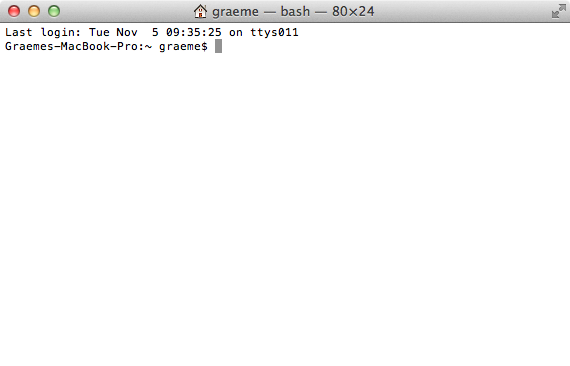
\includegraphics[scale=0.4]{terminal.png}}
\caption{The ``Terminal'' on an Apple computer - on a Windows computer
  this will look a little different.}
\end{figure}

\noindent
and they let you talk to the computer. All you need to do in here is type ``python'' and you should see

{\small
\begin{verbatim}
Python 2.7.3 (default_cci, Dec 13 2012, 05:32:36) 
[GCC 4.2.1 (Apple Inc. build 5666) (dot 3)] on darwin
Type "help", "copyright", "credits" or "license" for more information.
>>> 
\end{verbatim}
}

\noindent 
or something similar which says that the computer is ready to start
talking to you in Python. If you see this then everything is set up
just fine. 

\chapter{Pythons and Turtles}

\section{Introduction}

Most programming books begin with showing how to print something
(which means show it on the screen) usually ``Hello, World!'', and
then move on to how to print your name, numbers and so on. This is not
very interesting so this book will start with how to draw some shapes,
which is a good way of learning how to tell the computer things, as
you need to think hard about what you want first. For this we will use
the Python turtle. 

\section{The Python Turtle}

The Python turtle module (a module is a ``lump'' of computer program)
is a little arrow which you can use to draw pictures. Unlike most
drawing programs where you use a mouse to do drawing for this you need
to tell it where to go. The simplest way to use it is to tell it to go
forwards, backwards, left and right by certain amounts, and to lift
the pen up and to put it down again. When you start it is pointing
sideways. 

This is where you need to start thinking about \emph{exactly} what you
want the computer (or turtle) to do. Let's start by drawing a
square. Easy right? But you need to imagine that you are walking
around and holding a giant pen and blindfolded - how would you draw a
square then? This is the kind of instructions you need to give the
computer: 

\begin{enumerate}
\item{Step forwards 100 paces}
\item{Turn left}
\item{Step forwards 100 paces}
\item{Turn left}
\item{Step forwards 100 paces}
\item{Turn left}
\item{Step forwards 100 paces}
\item{Turn left}
\end{enumerate}

\noindent
if you do this you should find you have drawn a square about 100 paces to a side. We really need to be more specific though - how far left to turn? Also it's boring to repeat yourself like this, but we will come back to that later with something called \emph{loops}. 

Here's some Python code to do exactly this:

{\small
\begin{verbatim}
import turtle
turtle.forward(100)
turtle.left(90)
turtle.forward(100)
turtle.left(90)
turtle.forward(100)
turtle.left(90)
turtle.forward(100)
turtle.left(90)
\end{verbatim}
}

\noindent
If you type this into the Python window you should see a new white
square window pop up and a little white box will appear like
Figure~\ref{figure-turtle-001-square} and your Python window should looks like this:

{\small
\begin{verbatim}
Graemes-MacBook-Pro:~ graeme$ python
Python 2.7.1 (r271:86832, Jul 31 2011, 19:30:53) 
[GCC 4.2.1 (Based on Apple Inc. build 5658) (LLVM build 2335.15.00)] on darwin
Type "help", "copyright", "credits" or "license" for more information.
>>> import turtle
>>> turtle.forward(100)
>>> turtle.left(90)
>>> turtle.forward(100)
>>> turtle.left(90)
>>> turtle.forward(100)
>>> turtle.left(90)
>>> turtle.forward(100)
>>> turtle.left(90)
>>> 
\end{verbatim}
}

\begin{figure}
\label{figure-turtle-001-square}
\centering
\fbox{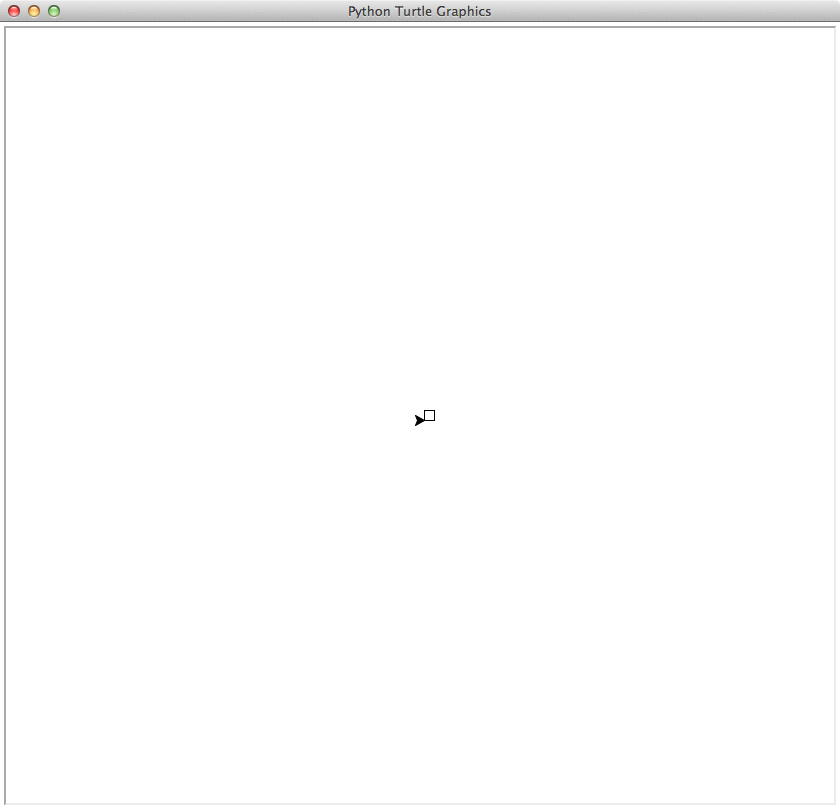
\includegraphics[scale=0.4]{turtle-001-square.png}}
\caption{The square drawn by the turtle after stepping forward 100 and
  turning left 90 four times.}
\end{figure}

What we have done here is to say first "I would like to use the turtle" then we have said four times to move forward 100 steps and to turn left by 90 degrees (which is a corner on a square.) You may find after you have typed all of this that you did not need to type it all, as Python remembers what you have done and so you can sometimes just press the "up" arrow on the keyboard and re-run some of the things you have typed already.

You can also lift the pen up with \verb|turtle.penup()| and put it down again with \verb|turtle.pendown()| - with these it is possible to draw some very fancy pictures limited only by your imagination and patience! Why not go and play some. When you've drawn some pictures ``by hand'' like this let's find out about loops.

\section{Loops}

Just to draw a square earlier took a lot of typing - when you are a
computer it can take a lot of instructions to do something
simple. There are easier ways to do this though, and one of them is to
have something called a loop. Loops are easy - they just say to do the
same thing over and over again. We could draw the square with a loop
like this (watching very carefully where the spaces go!)

{\small
\begin{verbatim}
import turtle
for j in range(4):
  turtle.forward(100)
  turtle.left(90)
\end{verbatim}
}

\noindent 
which tells the computer to do the same thing four times. It is useful to look at these lines one at a time. If you type \verb|range(4)| you will see \verb|[0, 1, 2, 3]| - this is what Python calls a list, and it is a list of numbers which go from 0 to 3. This is Python's way of counting which is a bit odd but you will get used to it. Then we have the \verb|turtle.forward(100)| command and the \verb|turtle.left(90)| command a little way in - there are two spaces in front. This says that these instructions are \emph{inside} the loop. If you do this you will find it draws exactly the same square as earlier. You can also have something like:

{\small
\begin{verbatim}
for j in range(4):
  print j
\end{verbatim}
}

\noindent 
which will just print the numbers from 0 to 3 (counting again) like this:

{\small
\begin{verbatim}
>>> for j in range(4):
...   print j
... 
0
1
2
3
\end{verbatim}
}

\noindent
What is happening here is that \verb|j| is set to 0, then the print command is done, then \verb|j| is set to 1 and the print command is done and do on. When we draw a square we don't use the \verb|j| for anything, but when we print it we do. The fun thing about loops though is we can do things a lot more than four times - what do you think

{\small
\begin{verbatim}
import turtle
for j in range(360):
  turtle.forward(1)
  turtle.left(1)
\end{verbatim}
}

\noindent
will do? Why not type it in and find out? And be sure to get those
spaces right! Also what about:

{\small
\begin{verbatim}
import turtle
for j in range(60):
  turtle.forward(j)
  turtle.left(90)
\end{verbatim}
}

Finally all of these examples assume you have started from a new
Python - if you want to use one which is going already just use:

{\small
\begin{verbatim}
turtle.reset()
\end{verbatim}
}

\noindent
which clears the screen - you also don't need to keep typing import
turtle as after the first time you already have it.

\subsection{Loops Inside Loops}

Sometimes there are things you want to do over and over (like drawing
a square earlier) which themselves require doing something over and
over (like drawing the sides of that square). Python allows you to do
all of this by having one loop (draw the sides of the square) inside
the other loop, for example:

{\small
\begin{verbatim}
import turtle

for i in range(10):
  for j in range(4):
    turtle.forward(10 * (i + 1))
    turtle.left(90)
\end{verbatim}
}

\noindent
This will give you something like
Figure~\ref{figure-loop-within-loop}, a series of squares each getting
larger than the last. This little program shows you two things - the
letters \verb|i| and \verb|j| here have to be different letters do the
program knows which one you mean, and you have to be very careful with
spaces (two, then four) as these tell the program which instructions
need to be performed within which loop.

\begin{figure}
\label{figure-loop-within-loop}
\centering
\fbox{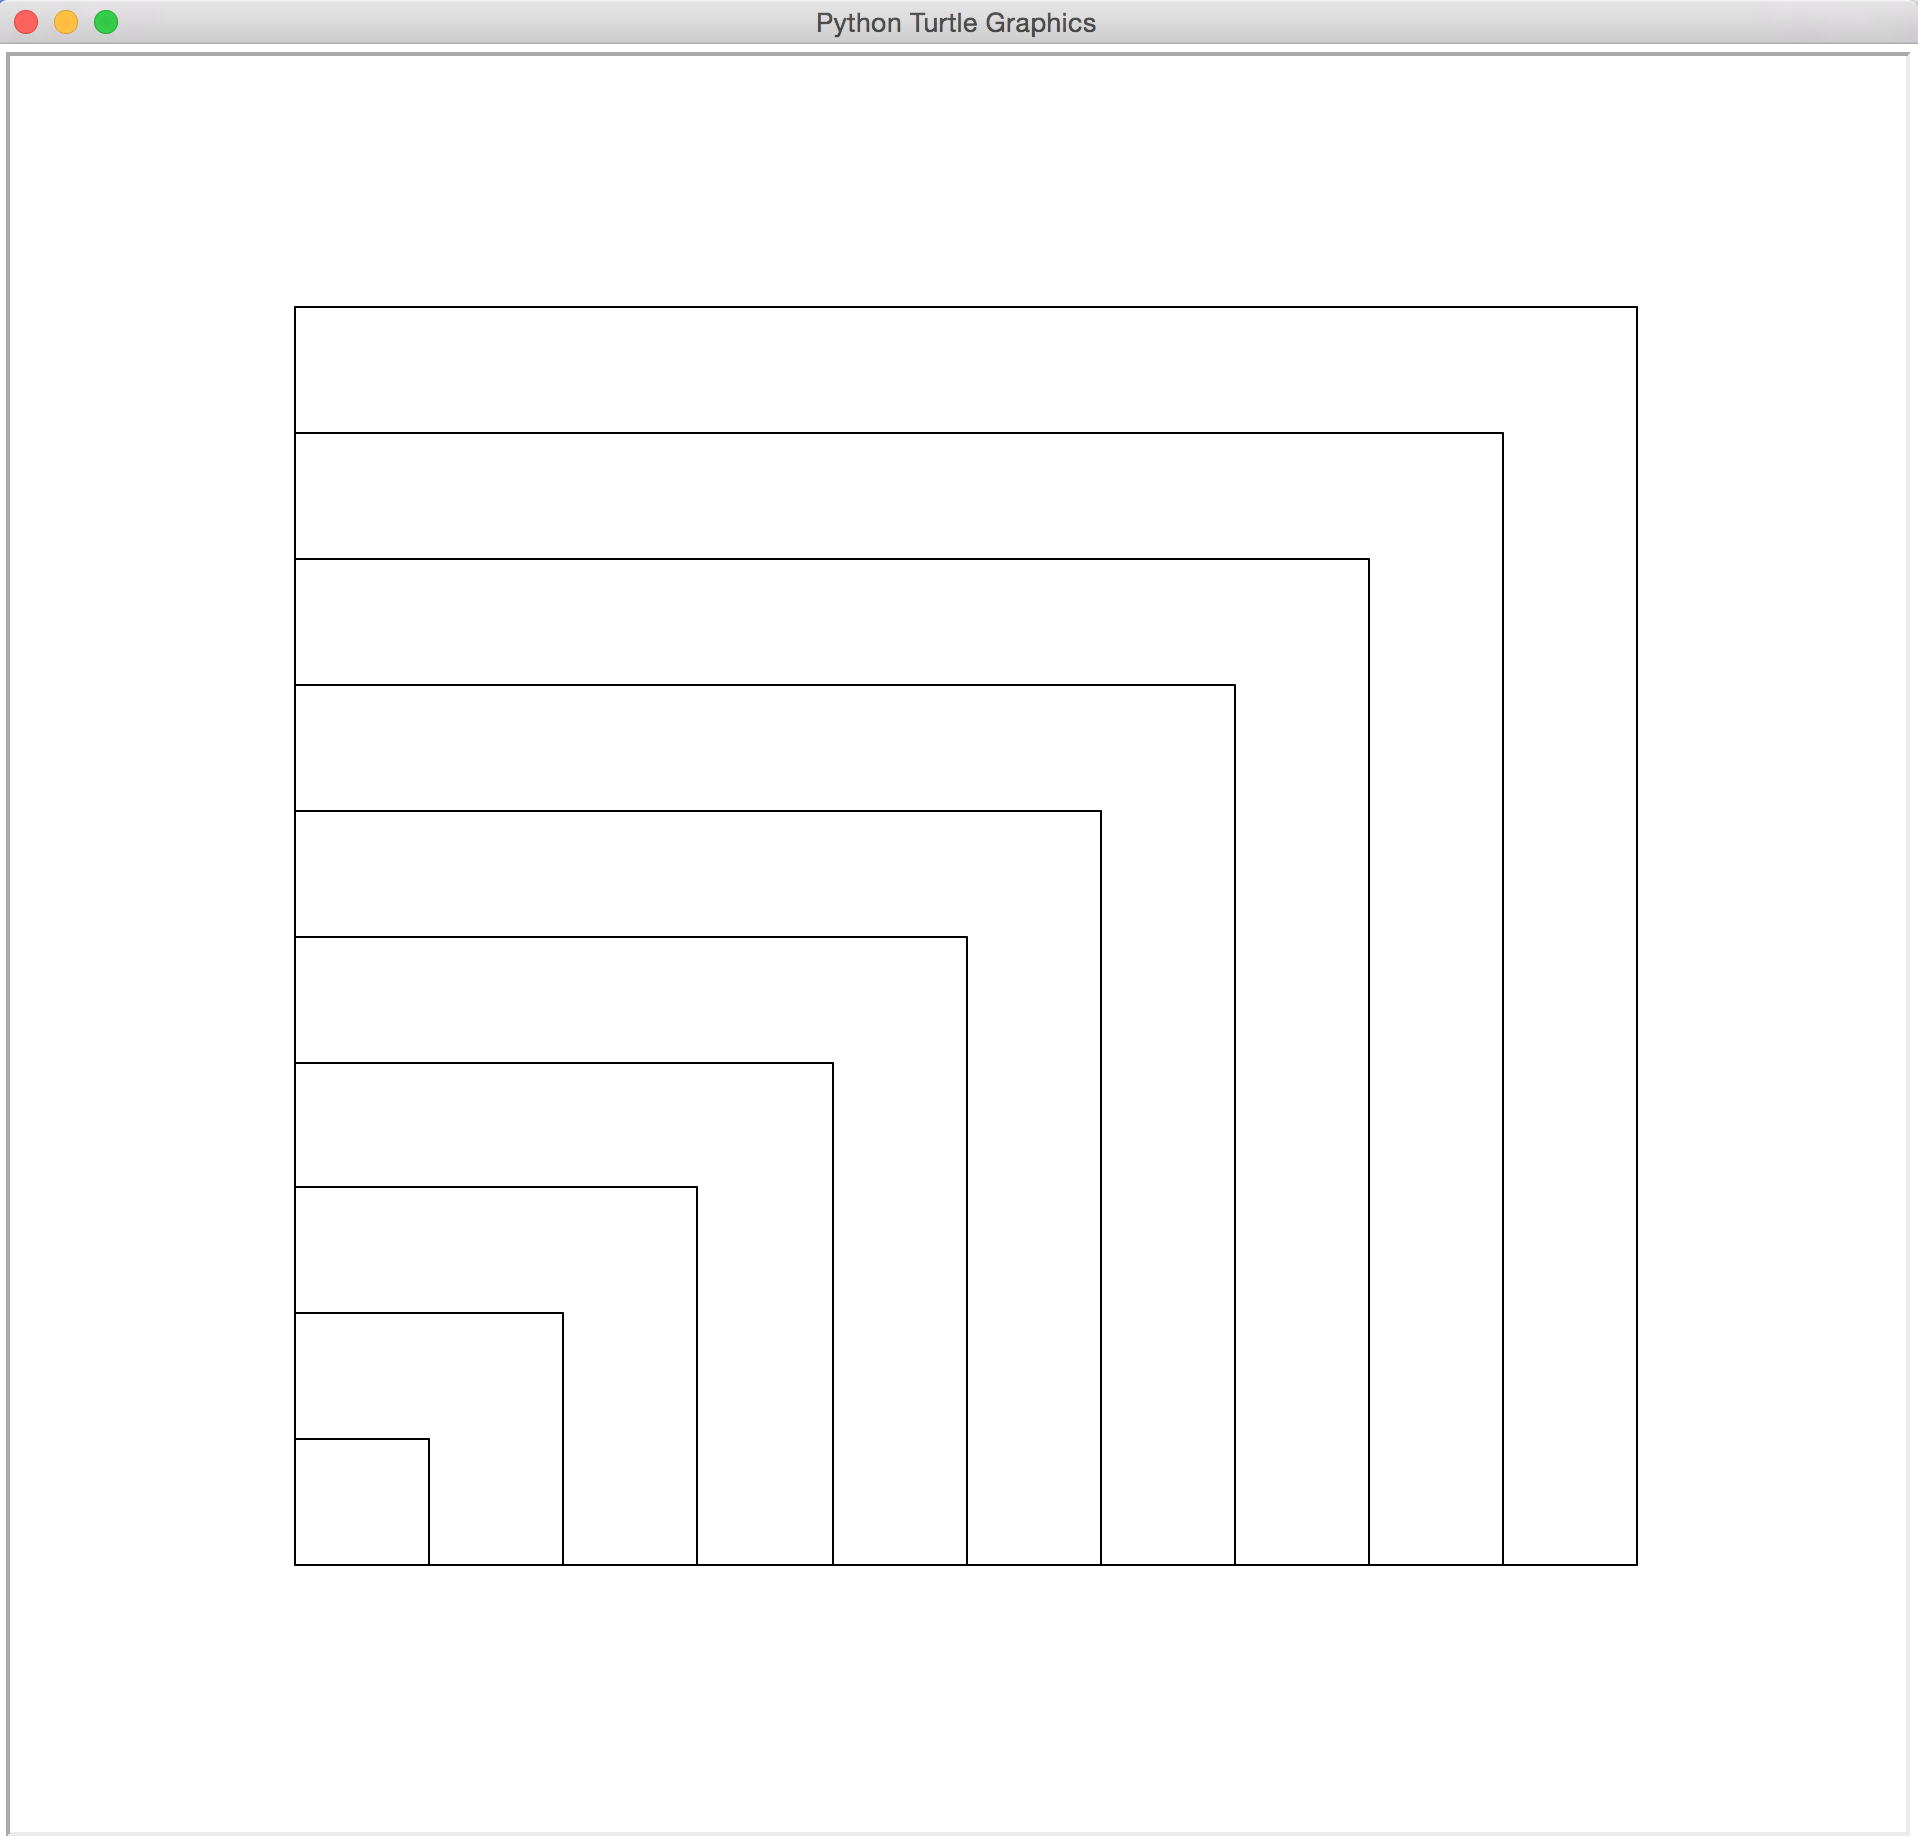
\includegraphics[scale=0.4]{turtle-001-loop-loop.png}}
\caption{A series of squares drawn by a loop within a loop.}
\end{figure}

This does however mean you can make some really fancy shapes like
Figure~\ref{figure-fancy}. The code for which will follow later...

\begin{figure}
\label{figure-fancy}
\centering
\fbox{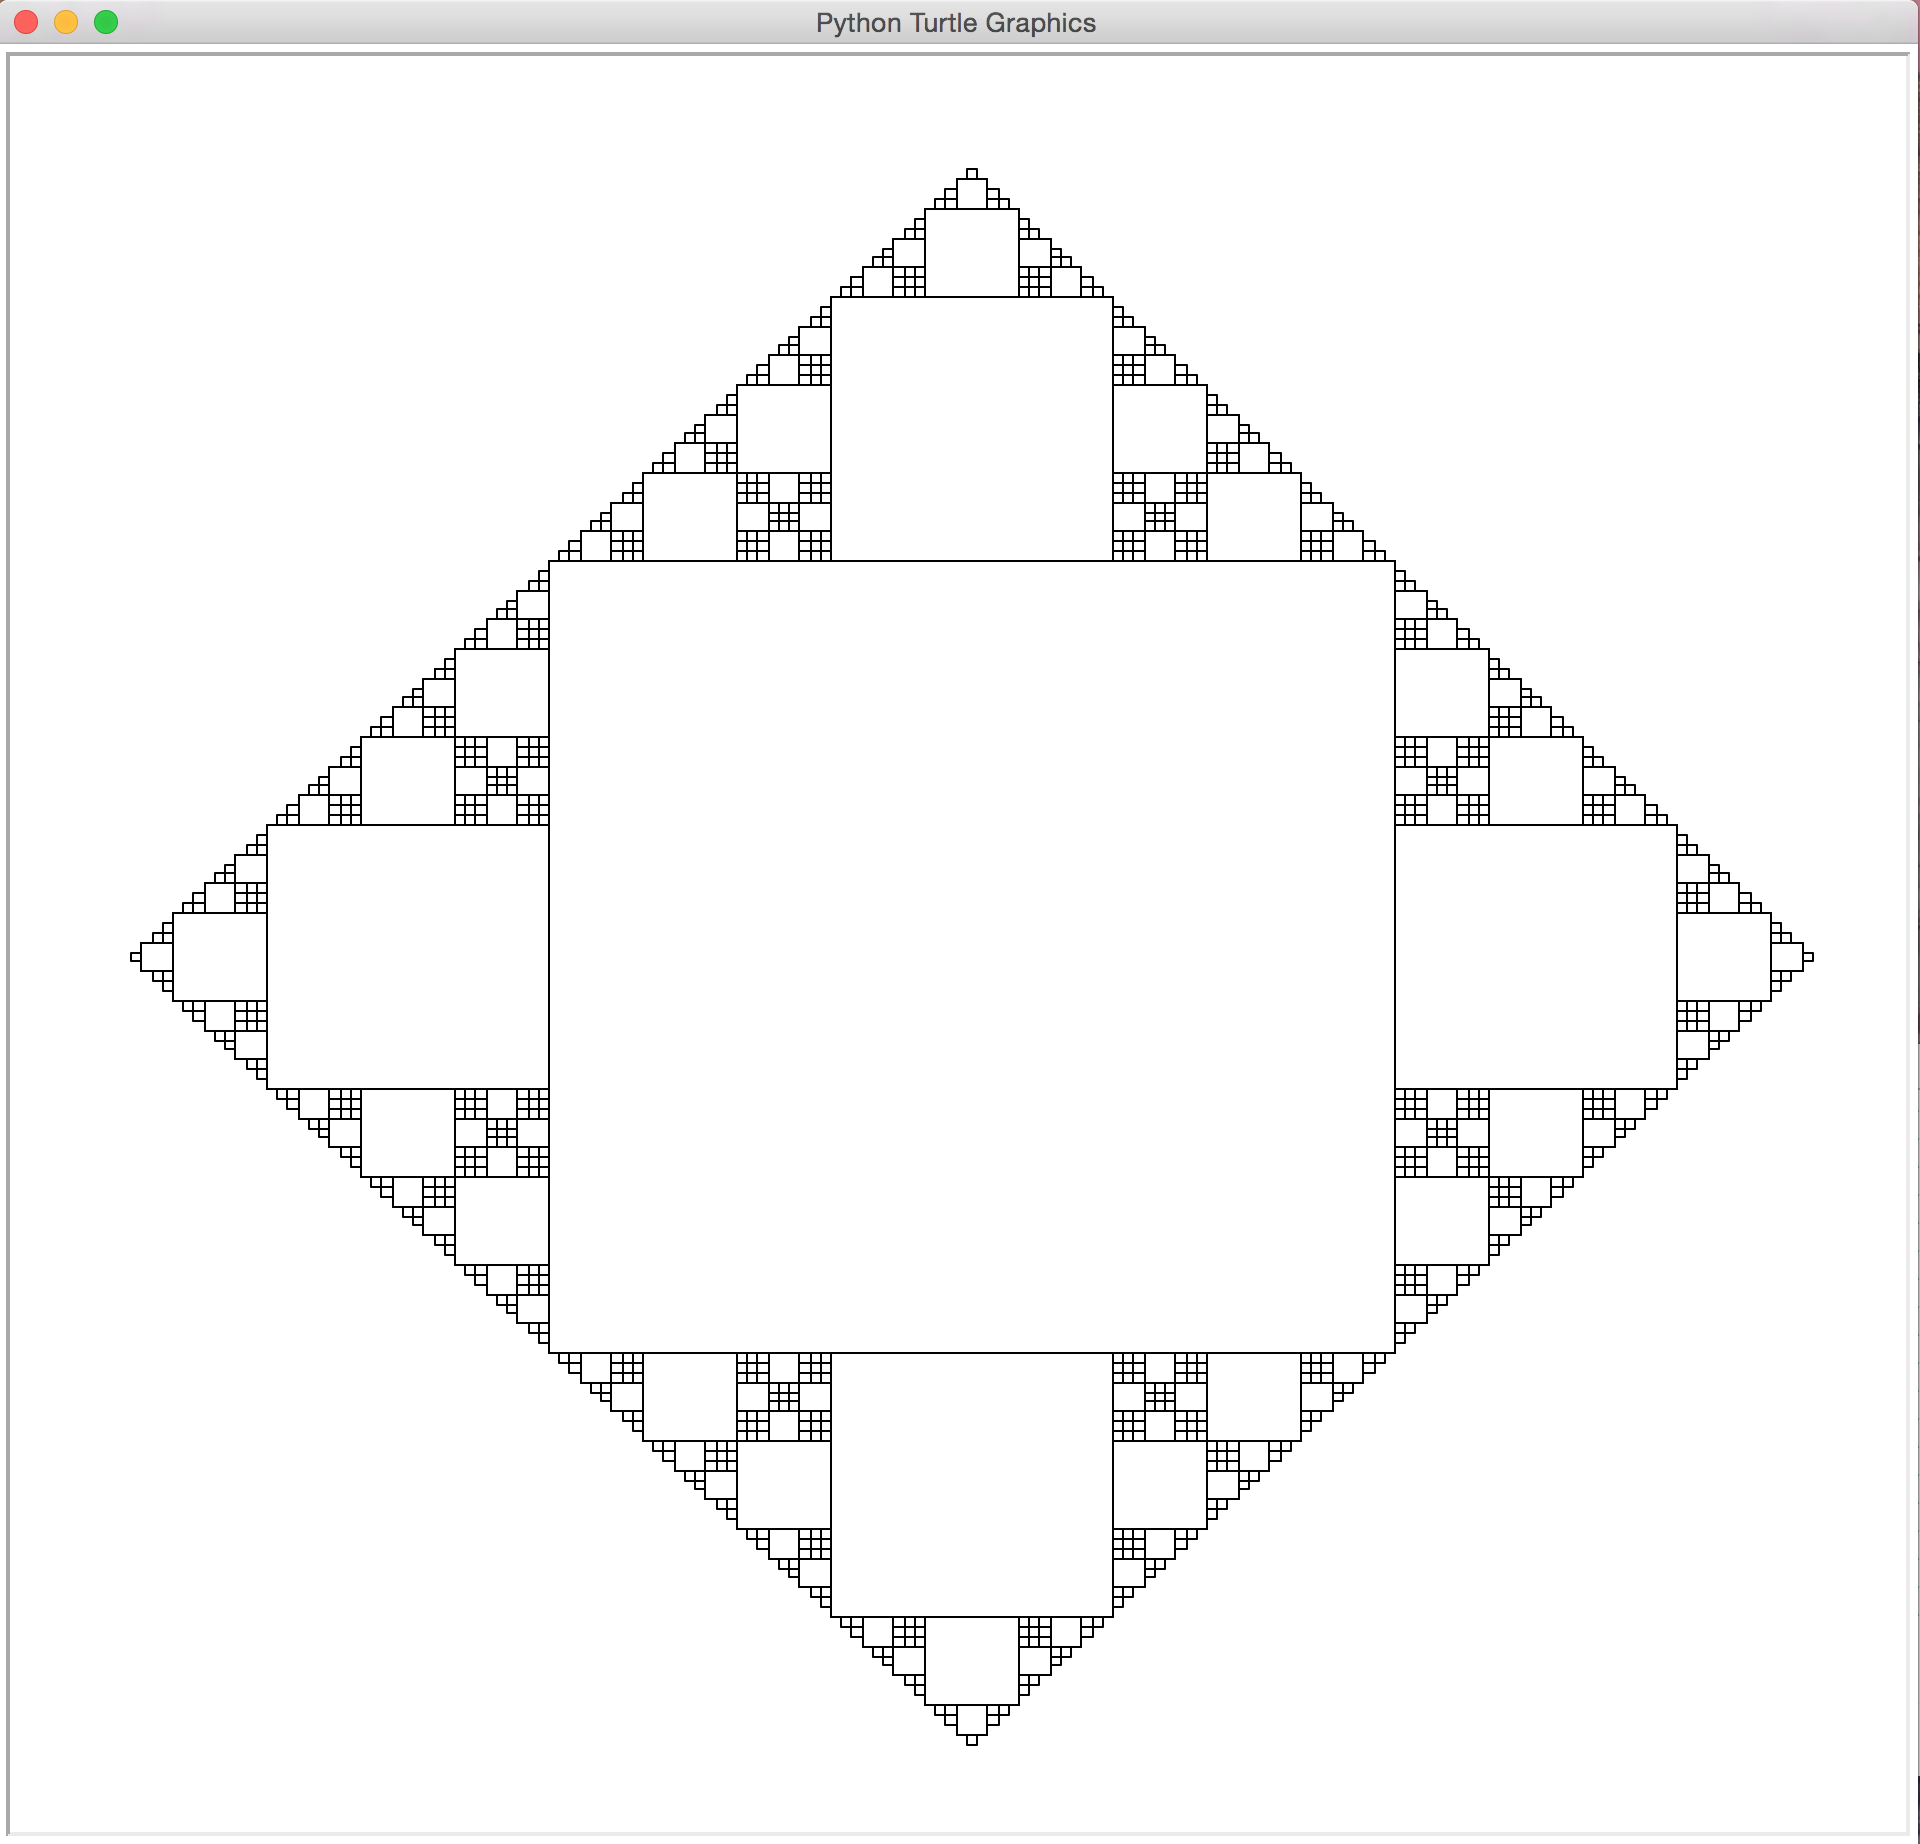
\includegraphics[scale=0.4]{turtle-fancy.png}}
\caption{What you can do with lots of loops!}
\end{figure}

\section{Mistakes}

Sometimes you will type things in wrong - this is fine and everyone does this - when you do make a mistake Python will complain that it does not understand, and usually this will have the word ``Error:'' in the message and it will try to explain what was wrong. When you have done this a lot you will find that these messages make sense but right now don't worry.

{\small
\begin{verbatim}
>>> import turtle
>>> for j in range(360):
...   turtle.forwards(1)
...   turtle.left(1)
... Traceback (most recent call last):
  File "<stdin>", line 2, in <module>
AttributeError: 'module' object has no attribute 'forwards'
\end{verbatim}
}

\chapter{Programming Python}

In this chapter we will start to look at some of the elements which go
into writing a computer program, in particular variables, comparisons
and functions.

\section{Variables}

We have already been using a lot of variables but have not considered
what they actually are. In this code:

{\small
\begin{verbatim}
>>> for j in range(4):
...   print j
... 
0
1
2
3
\end{verbatim}
}

\noindent
\verb|j| is a variable. A variable is something which can be set to
some value, but we don't know what that value is. For example, 2 is
always equal to 2 - it's never 1, 3.5 or 17. This means it's
constant. If I have something like \verb|a = 2| however it means
\emph{right now} \verb|a| is equal to 2 but later we could set it to
something else. This is very useful for writing computer programs as
we know what we want to do, but sometimes we don't know what we want
to do it to, for example priting your name:

{\small
\begin{verbatim}
Graemes-MacBook-Pro-2:python_for_under_10s graeme$ python
Python 2.7.8 (default_cci, Mar 19 2015, 08:06:01) 
[GCC 4.2.1 Compatible Apple LLVM 6.0 (clang-600.0.57)] on darwin
Type "help", "copyright", "credits" or "license" for more information.
>>> name = raw_input('--> ')
--> Graeme
>>> print name
Graeme
\end{verbatim}
}

Here we know \verb|raw_input| will get your name (or whatever else you
typed in) but we don't know what that is. It doesn't matter though, we
can still print it. We can also get Python to \emph{guess} your name
with this:

{\small
\begin{verbatim}
import getpass
print getpass.getuser()
\end{verbatim}
}

This will print the name of the person who is logged in, who could be
you, or your mum or dad, or some other name completely! We can use
this name like this:

{\small
\begin{verbatim}
import getpass
name = getpass.getuser()
print name
\end{verbatim}
}

\noindent
which says to get the user name then save it for later use in the
\emph{variable} \verb|name|.

\section{Comparisons}

Sometimes we may want do to something special if the value of some
variable is equal to something, or bigger than it or less than
it. Making a decision about this is called a \emph{comparison} as we
are comparing a variable with something. In Python this works like
this:

{\small
\begin{verbatim}
a = 1
if a == 2:
  print 'Something strange as happened!'
\end{verbatim}
}

\noindent
where we set \verb|a = 1| then act surprised (we should be really
surprised) if in the next line it is suddenly 2! Something could
happen to a in the meantime though like this:

{\small
\begin{verbatim}
a = 1
a = 2 * a
if a == 2:
  print 'Something strange as happened!'
\end{verbatim}
}

\noindent
so now we would expect it to print something - the strange thing is a
was multiplied by 2. This can be more fun if we change the behaviour of
the program depending on the value of a variable:

{\small
\begin{verbatim}
import getpass
name = getpass.getuser()
if name == 'graeme':
  print name, 'smells!'
else:
  print name, 'is nice'
\end{verbatim}
}

Here if the name logged into the computer is \verb|graeme| one thing
will happen, otherwise something else will happen. Combining this kind
of thing with loops can start to make some much more interesting
things happen.

\section{Functions}

In this example code

{\small
\begin{verbatim}
import getpass
name = getpass.getuser()
print name
\end{verbatim}
}

\noindent
and in lots of other places you have seen brackets \verb|()| at the
ends of words. These sometimes have things \verb|(in, them)| and we
used them a lot for the turtle like \verb|turtle.forward(100)|. These
brackets mean that we have called a \emph{function} which means in
computer speak ``go and find this code and do what it says.'' This is
how most programming works including the turtle - people write code
which other people can then use to make programs. The fancy picture in
the previous chapter was made using functions, and variables, and
looks like this:

{\small
\begin{verbatim}
import turtle

def draw(itrn):
  sqr = 'FRFRFRFR'
  for j in range(itrn):
    sqr = sqr.replace('F', 'FLFRFRFLF')
    
  for s in sqr:
    if s == 'F':
      turtle.forward(3 ** (4 - itrn))
    elif s == 'L':
      turtle.left(90)
    elif s == 'R':
      turtle.right(90)

for j in range(5):
  draw(j)
\end{verbatim}
}

\end{document}
